\chapter{Le premier principe de la thermodynamique} 
Également connu sous le doux nom de \textit{principe de 
conservation de l'énergie}, il s'agit d'un postulat fondamental
qui ne se démontre pas.

\section{Transformations fermées (cycles) d'un système fermé}
Soit le système fermé ci-dessous :
\begin{center}
	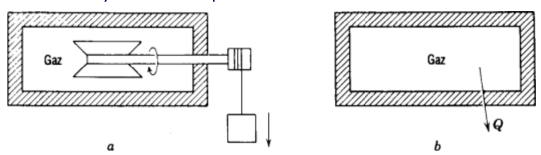
\includegraphics[scale=0.5]{ch5/image1}
	\captionof{figure}{ }
\end{center}
On travaille en deux temps :
\begin{enumerate}
	\item On fournit un travail $W$ au système.
	\item On le laisse revenir à son état initial par échange de $Q$.
\end{enumerate}
Ces deux transformations constituent un cycle. Le premier principe 
postule que\\

\retenir{Le travail $W$ et la chaleur $Q$ échangés au cours d'un 
	tel cycle sont proportionnels, la constante de proportionnalité 
	étant toujours la même.
	\begin{equation}
		JQ = W \qquad \Leftrightarrow \qquad J\oint \delta Q = \oint \delta 
		W
	\end{equation}
	où $J$, la constante de $\propto$ dépend des unités utilisées.}\ \\

Si $Q$ et $W$ sont dans la même unité, cette constante vaut -1 et 
l'expression du premier principe devient
\begin{equation}
	\oint (\delta Q + \delta W) = 0
\end{equation}

\section{Transformation ouvertes d'un système fermé}
Soit un système fermé subissant un cycles formé de deux transformations 
successives $A$ et $B$. En vertu du premier principe :\\
\begin{wrapfigure}[9]{l}{6cm}
	\vspace{-7mm}
	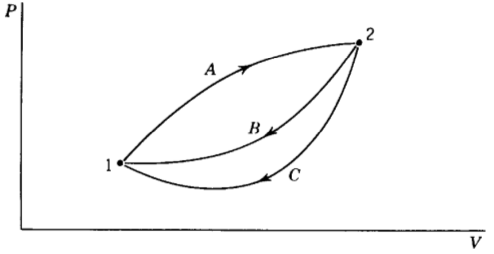
\includegraphics[scale=0.34]{ch5/image2.png}
	\captionof{figure}{ }
\end{wrapfigure}
\vspace{-1cm}
\begin{equation}
	\oint (\delta Q + \delta W) = \int_1^2 (\delta Q + \delta W)_A + \int_2^1 
	(\delta Q + \delta W)_B = 0
\end{equation}
De même, pour le cycle formé par $A$ et $C$ :
\begin{equation}
	\int_1^2 (\delta Q + \delta W)_A + \int_2^1 (\delta Q + \delta W)_C = 0
\end{equation}
Par soustraction, en en déduit que
\begin{equation}
	\int_1^2 (\delta Q + \delta W)_B = \int_1^2 (\delta Q + \delta W)_C
\end{equation}
Les chemins $B$ et $C$ sont arbitraires, l'intégrale est indépendante 
du chemin parcouru : $(\delta Q + \delta W)$ est une différentielle 
exacte que l'on désigne :
\begin{equation}
	dE = \delta Q + \delta W
\end{equation}
où $dE$ est l'\textbf{énergie du système}. En intégrant de l'état 1 à 
l'état 2, on obtient
\begin{equation}
	\ _1Q_2 + \ _1W_2 = E_2-E_1
\end{equation}
Cette énergie peut être cinétique, potentielle, chimique, \dots En 
thermodynamique, on sépare les énergies cinétiques et potentielles 
des autres\footnote{Car elles dépendent du référentiel et s'expriment 
	en fonction de la masse, de la vitesse et des coordonnées dans ce 
	référentiel.} qui sont regroupées dans une variable $U$, l'\textbf{
énergie interne}.
\begin{equation}
	dE = dU + dE_{cin.} + dE_{pot.}
\end{equation}
La forme différentielle du premier principe s'exprime :
\begin{equation}
	\delta Q + \delta W = dU + dE_{cin.} + dE_{pot.}
\end{equation}
Après substitution des expression bien connue grâce aux cours de \textit{
Mécanique rationnelle I/II} : 
\begin{equation}
	\delta Q + \delta W = d\left(\frac{mc^2}{2}\right) + d(mgz)
\end{equation}
En intégrant entre les états initial et final (si $g$ est constante)
\begin{equation}
	\ _1Q_2 + \ _1W_2 = U_2 - U_1 + m\frac{c_2^2-c_1^2}{2}+mg(z_2-z_1)
\end{equation}
Ces équations n'informent que sur les variations d'énergie qui sont 
donc définie à une constante près.

\section{L'énergie interne}
La variable $U$ est extensive et on peut dès lors lui associer une 
variable extensive